\documentclass[man,noapacite,12pt]{apa2}
\usepackage{amsmath}
\usepackage{booktabs}
\usepackage{apacite2}
\usepackage{fullpage,rotating}
\usepackage{pslatex}
\usepackage{amssymb}
\usepackage{accents}

% \usepackage{synctex}

\newcommand{\vect}[1]{\accentset{\rightharpoonup}{#1}}

\title{Learning word meaning by inferring speakers' intentions: \\ An incremental approach to socially-guided statistical learning}

\author{Michael C. Frank, Molly L. Lewis, Mika Braginsky, \& Noah D. Goodman}
\affiliation{Department of Psychology, Stanford University}

\shorttitle{Learning words by inferring reference}
\rightheader{Learning words by inferring reference}


\acknowledgements{Many thanks to ...

~

\noindent Please address correspondence to Michael C. Frank, Department of Psychology, Stanford University, 450 Serra Mall (Jordan Hall), Stanford, CA, 94305, tel: (650) 724-4003, email: \texttt{mcfrank@stanford.edu}.}


\abstract{How do children learn the meanings of words? While some accounts suggest that word learning happens in a single moment, others privilege the gradual accumulation of information across time. Previous modeling work has attempted to unify these viewpoints in a single framework that allows for both in-the-moment interpretation and gradual statistical accumulation, but at the cost of substantial computational complexity. We describe a new, incremental model of this interaction, in which statistical associations are the product of in-the-moment interpretations. This process-level model successfully captures a number of experimental findings (including some that were not captured by previous, computational-level analyses) and suggests a number of extensions.}

\begin{document}
\maketitle                            


\section{Introduction}

Word learning is a fundamental part of language acquisition. Starting slowly in late infancy and speeding up after their first birthday, children accumulate a vocabulary of words that they can reliably recognize and produce \cite{bergelson2012,bloom2002}. The exact timing of this process is highly variable across children, but generally by the end of the second year, children can produce several hundred words and are well on their way to combining these to express complex and novel propositions \cite{brown1973,fenson1994}. How are these early words learned? 

In this paper, we elaborate an answer to this question that combines children's statistical learning abilities \cite{saffran1996b,aslin2012} with their emerging competence in social interaction \cite{carpenter1998}. Our proposal is that vocabulary is accumulated via a process in which children attempt to interpret the language they hear, and then retain guesses about the meanings of words based on these interpretations. Building on a previous model of joint interpretation and language learning \cite{frank2009}, we implement this proposal in the language of probabilistic modeling. Our model instantiates the idea that there are two timescales involved in word learning \cite<cf.>{mcmurray2012}: in-the-moment interpretation, and cross-situational mapping. 

Our model constitutes an incremental approach to integrating across timescales: For each utterance, it proposes a possible referential interpretation, then updates a graded lexicon accordingly. Although the model is incremental, it nevertheless instantiates normative Bayesian inferences; in this respect it is a ``rational process model'' that makes normative probabilistic inferences under cognitive resource constraints \cite{griffiths2012,sanborn2010}. We compare this incremental, process-level inference algorithm with a batch inference algorithm that considers all the available data and find that they are surprisingly similar to one another. One radical consequence of this approach is that there is no separate process of ``word learning''; instead word learning is what falls out of learners remembering their best guesses about what a particular piece of language meant in the contexts of its use.

In what follows, we briefly motivate our proposal with respect to the previous literature on children's word learning. We then review prior computational models of word learning with the goal of grounding and highlighting our conceptual contributions. We then present our model and show that it can be both applied to annotated corpora of child language and can be used to simulate individual experiments. We end by considering open questions for the field of early language learning.

\subsection{Mechanisms of early word learning}

One clue to the mechanisms of early vocabulary learning comes from the makeup of children's early vocabulary. Although children produce words of all different types, certain kinds of words are nevertheless overrepresented in early vocabulary. Names for things make up a substantially larger proportion of children's early vocabulary than they do later \cite{tardif2008,caselli1995}, alongside names for people and and words used in simple social routines (e.g., ``hi'' and ``bye''). Many observers have suggested that these kinds of words---especially basic-level nouns---are learned early because of the ease with which the linguistic form can be mapped to a particular observable referent \cite{locke1700,bloom2002,clark2003}. From there, generalizing particular referents to a broader class of referents is relatively trivial, given that the relevant concepts are typically at the basic-level and typically represent whole objects rather than parts \cite{markman1991}.

A single learning instance can in principle provide strong evidence for a particular word meaning. For example, imagine that a parent points to a ball and says ``ball!'' An observer with an understanding of pointing can infer that the speaker is referring to the ball, infer that the concurrently uttered word refers to it, and generalize to the broader concept of balls in general. In practice, however, very young children typically require several exposures to a word before they recognize it and retain it for future use, even when the context of naming is unambiguous \cite{woodward1994}.

In addition, many learning situations range from slightly to substantially more ambiguous. Imagine that the parent had uttered the phrase ``look at that nice, round ball!''---this phrase has a number of competing words that might be candidates for the object name (though perhaps worse candidates by virtue of sentential position, stress, or phonological structure). Or the parent might not have pointed but instead relied on the fact that the child was playing with the ball. Perhaps there might have been other toys present competing for the child's attention. In each of these cases, the child might be able to guess that the word ``ball'' referred to the ball, but with less certainty than in the simplest case \cite<>[gives a concrete instantiation of such differences in certainty in naturalistic play session videos]{yurovsky2013}. 

While such ambiguous cases might not license strong inferences about word meaning, many theorists have noted that learners in principle could accumulate information across instances \cite{pinker1984,gleitman1990,siskind1996,yu2007}. This strategy, dubbed \emph{cross-situational learning}, has now been demonstrated in a number of small-scale laboratory experiments with both adults and children \cite{yu2007,smith2008}. In addition, a number of computational demonstrations suggest that this kind of strategy could be effective for learning in social situations \cite{yu2007b,frank2009,johnson2012}, with realistic vocabulary sizes and levels of ambiguity \cite{blythe2010}, and even with more complex propositional meanings \cite{siskind1996}. In fact, a growing literature in natural language processing implements precisely this strategy for a variety of what are known as ``grounded language learning'' tasks \cite<e.g.>{zettlemoyer2005,wong2007,artzi2013,liang2011,kim2013}.

Nevertheless, the existence of such an uncertainty-reduction strategy does not necessarily imply that learners make use of it. Indeed, there has been substantial debate about the degree to which learners represent cross-situational statistics \cite{medina2011,yu2012,yurovsky2013,trueswell2013,smith2011b,yurovskyunderreview}. On some accounts, learners encode only a single hypothesis at a time; on others, learners maintain some representation of all of the data that they have access to. But regardless of the specific representation and algorithm that learners use for this process, all accounts of cross-situational learning posit \emph{consistency} across situations, which even single-hypothesis learners exploit by checking their hypotheses across situations \cite{trueswell2013,yu2012}. To understand the range of possible theories of cross-situational learning, we next turn to the modeling literature. 

\subsection{Prior modeling work}

Although a number of theorists had discussed cross-situational strategies for learning word meanings \cite{pinker1984,gleitman1990}, an important early instantiation of this idea came from a model by \citeA{siskind1996}. This model used a propositional representation of meaning in combination with a set of deductive rules to infer word-meaning mappings from artificial data. This ambitious model provided a powerful proof-of-concept, but was limited by the assumption that the propositional structure of meanings was observed by the learner. 

An alternate, more graded, view of word learning came from the connectionist tradition. \citeA{plunkett1992} described a graded word-image mapping model that reproduced a number of category generalization and vocabulary growth phenomena. This basic model type has been followed by a number of related models that capture phenomena like mutual exclusivity \cite{regier2005}, the phonological dynamics of the mono- and bilingual lexicon \cite{li2002,li2004,li2007}, and the emergence of categorization principles \cite{mayor2010}. Nevertheless, none of these models focused specifically on the challenge of disambiguating reference in ambiguous contexts. 

The problem of referential uncertainty played a more central role in a number of other models that emerged from the machine learning tradition. In a series of systems, Yu and colleagues developed a model stemming from classic machine translation systems \cite{brown1993}. This model looked for correspondences between words and their referents that was consistent across situations; these mappings could be biased by a number of perceptual and social aspects of the learning scenario \cite{yu2005,yu2007}. Critically, these models could be applied to annotated corpora of child-directed speech, a major advance over previous work that had only been applied to artificial corpora. 

A complementary probabilistic model considered how generalization biases could emerge from statistical inferences under ambiguity across situations \cite{xu2007}. This model was able to predict adults' and children's patterns of taxonomic generalization by reference to general principles of probabilistic inference. Although it did not specifically apply to the problem of referential uncertainty across situations, it nevertheless aggregated information across exposures to make graded inferences about word meaning. 

Building on these two lines of work, we proposed a probabilistic treatment of referential uncertainty in \citeA{frank2009}. This model differed from earlier approaches in that it explicitly assumed that in any individual situation, speakers have an intention to refer to a particular object or objects and that the labels they utter correspond to these words. In contrast, previous models had computed associations directly between words and referents, without considering that some of these associations were not relevant because the speaker might not be trying to refer to some objects. This ``intentional'' assumption led to an increase in accuracy in learning from corpus data relative to previous work, and also allowed the model to capture a number of experimental findings. A number of related pieces of work have extended this model to incorporate word segmentation \cite{johnson2010}, social cues \cite{frank2008,johnson2012}, conceptual generalization \cite{lewis2013b}, lexical constraints \cite{lewis2013}, some basic aspects of grammatical structure \cite{johnson2010}, and even pragmatic inference \cite{smith2013}.

The basic framework described in \citeA{frank2009} nevertheless suffered from a number of weaknesses. First, it posited a discrete lexicon represented by a bipartite graph linking words and object concepts. While this representation was technically convenient, it seemed at odds with the conception of graded, uncertain mappings implied by the experimental literature.\footnote{Although there is debate about the uncertainty implied by adult cross-situational learning experiments \cite<e.g.>{smith2012,trueswell2013}, many experiments with children imply increases in word recognition accuracy with greater experience \cite<e.g.>{fernald1998,bergelson2012}. Thus, some sort of graded conception of the lexicon appears to be an important aspect of models that hope to capture such findings.} In addition, the model was posed at Marr's \citeyear{marr1982} ``computational theory'' level; as such, it considered all the available data in its computation. This ``batch'' inference was of course unrealistic in terms of the memory constraints on leaners; in addition, practically speaking it kept the model from considering phenomena that involved the gradual accumulation of data about a particular inference. Finally, because of technical limitations, the inference scheme in this model was not fully Bayesian: It did not recover the posterior probability distribution on lexicons given a particular exposure. Instead, it only searched for the single best lexicon. 

One important parallel development has come from expansions of the \citeA{yu2007} translation model. \citeA{fazly2010} described an incremental version of this model, which they applied to meaning representations derived from speech in CHILDES. This model reproduced a number of empirical findings in the incremental context. In addition, the meaning representations were graded distributions over the full inventory of lexical elements. Both of these desirable features point the way towards applications of this model;  indeed, it has been extended to simulate cognitive constraints \cite{nematzadeh2012}, individual differences in acquisition \cite{nematzadeh2011}, and the effects of syntactic structure \cite{alishahi2010}.  Nevertheless, this model has no obvious route for the accommodation of social information. 

A second important development in incremental modeling of cross-situational learning is the model described by \citeA{mcmurray2012}. These authors introduce a connectionist model that---like the \citeA{frank2009} model---explicitly operates at two timescales: the timescale of language interpretation in the moment and the timescale of cross-situational mapping. Because of the incremental nature of this model, however, it is able to simulate the dynamics of reference resolution in the moment. In addition, the exhaustive set of simulations using this model suggests that the combination of graded representation, incremental processing, and multi-timescale inference allows this model to captures most of the relevant data points. Similar to the \citeA{fazly2010} model, however, the one major lacuna in this set of simulations is social learning phenomena. 

\subsection{The current model}

Taken together, the models presented by \citeA{frank2009}, \citeA{fazly2010}, and \citeA{mcmurray2012} synthesize and unify a striking amount of work on the mechanisms and dynamics of early word learning. Each of these has some features that could be improved upon, however. In particular, the \citeA{frank2009} model is non-incremental, while the \citeA{fazly2010}, and \citeA{mcmurray2012} models fail to consider social information. Our goal in the current work is thus to provide an incremental interpretation of the \citeA{frank2009} model, which would serve to unify the social framework in that work with the findings of these other incremental models.

\section{Model}


In the sections that follow, we describe the formal specification of our model as well as two inference algorithms---a batch Gibbs sampler and an incremental particle filter. As will become clear, these two inference algorithms are deeply related to one another. All code and data for the model and simulations reported below are available at \url{http://github.com/mcfrank/dmww}. 

\subsection{Model Specification}

\begin{figure}[tr]
\begin{center}
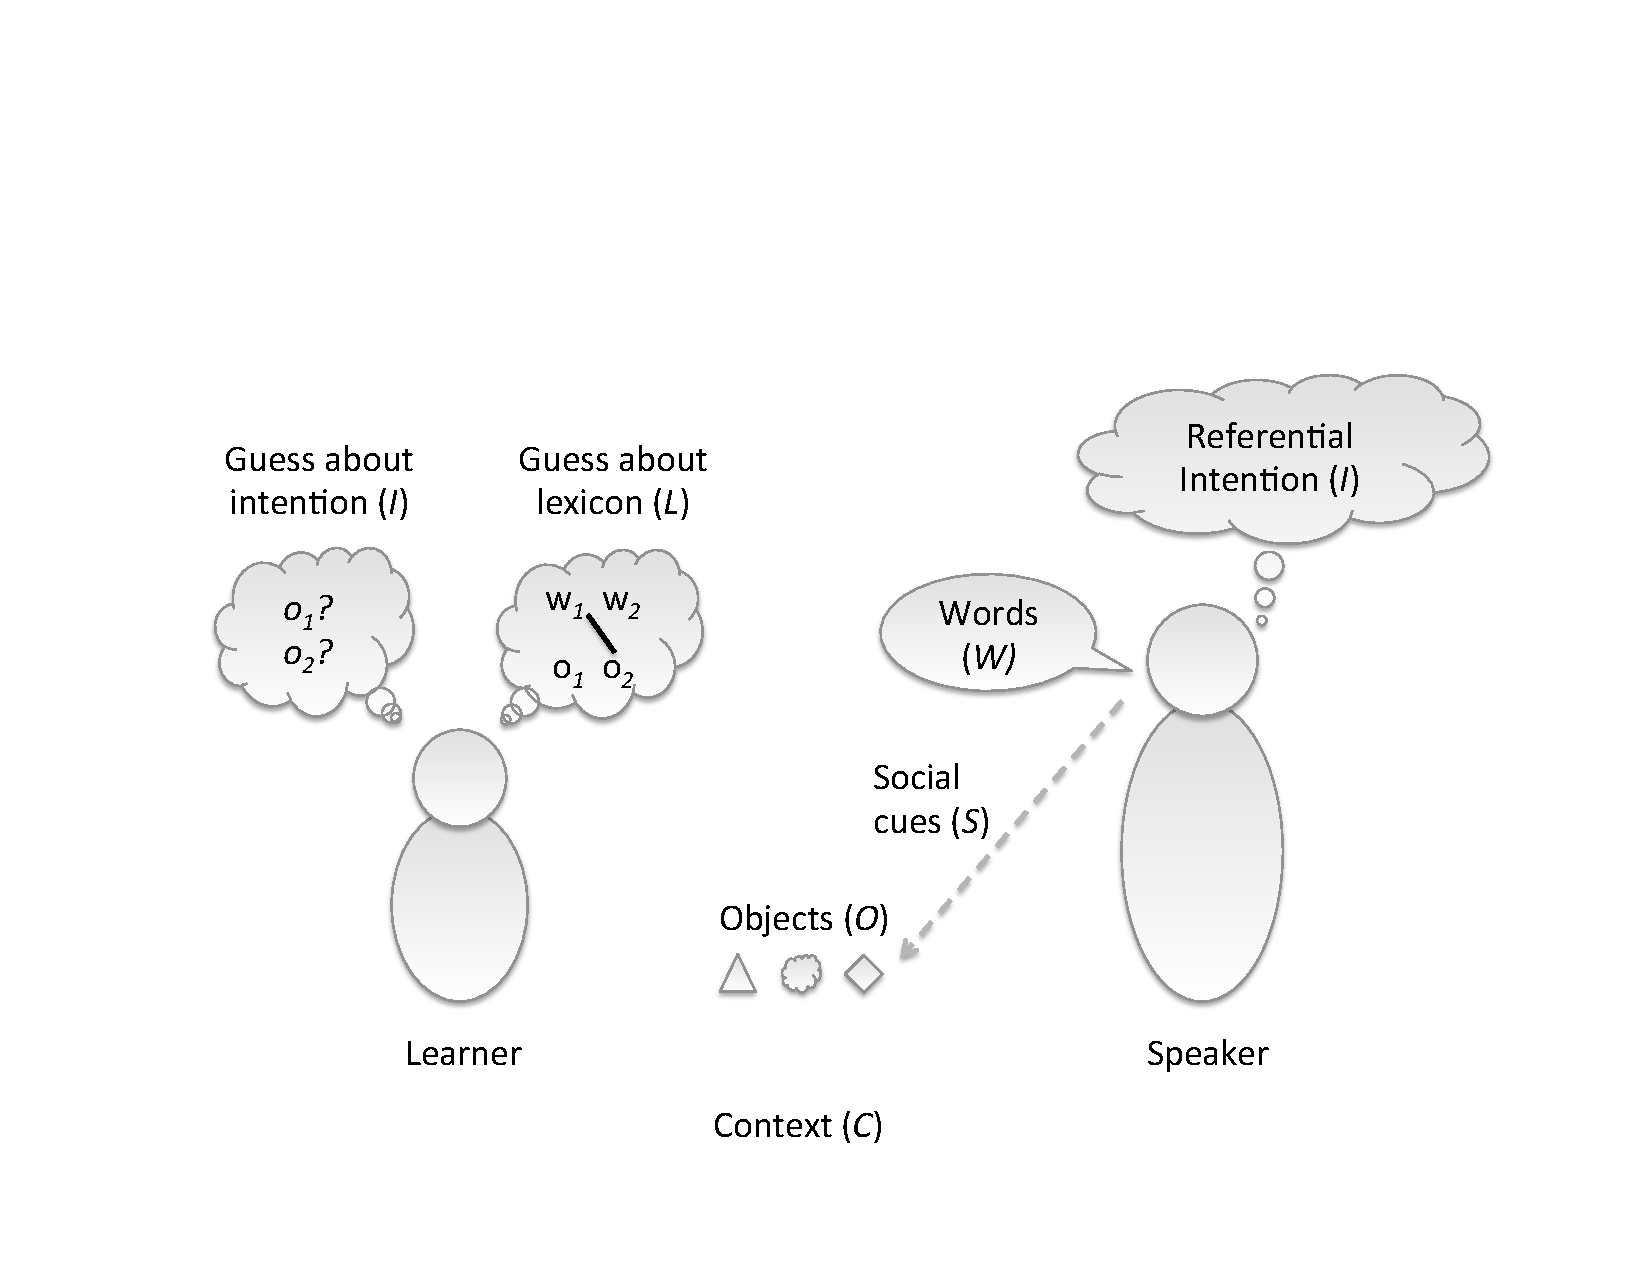
\includegraphics[width=4.5in]{figures/framework_mod.pdf}
\caption{\label{fig:setup} A schematic depiction of the learning situation, with the relevant variables marked for ease of interpretation. The learner faces a joint inference problem: inferring what the speaker is talking about and learning the consistent meanings of words. Reprinted from \protect\citeA{frank2014chap}.}
\end{center}
\end{figure}

The schematic word learning situation is shown in Figure \ref{fig:setup}. The learner is hypothesized to make join inferences in each situation about the speaker's referential intention $I$ and the lexicon of their language $L$, in the context $C$. These guesses are informed the elements of the context, the words $W$ that the speaker utters and the relevant referents (objects $O$) that are present in the situation. 


\begin{figure}[tr]
\begin{center}
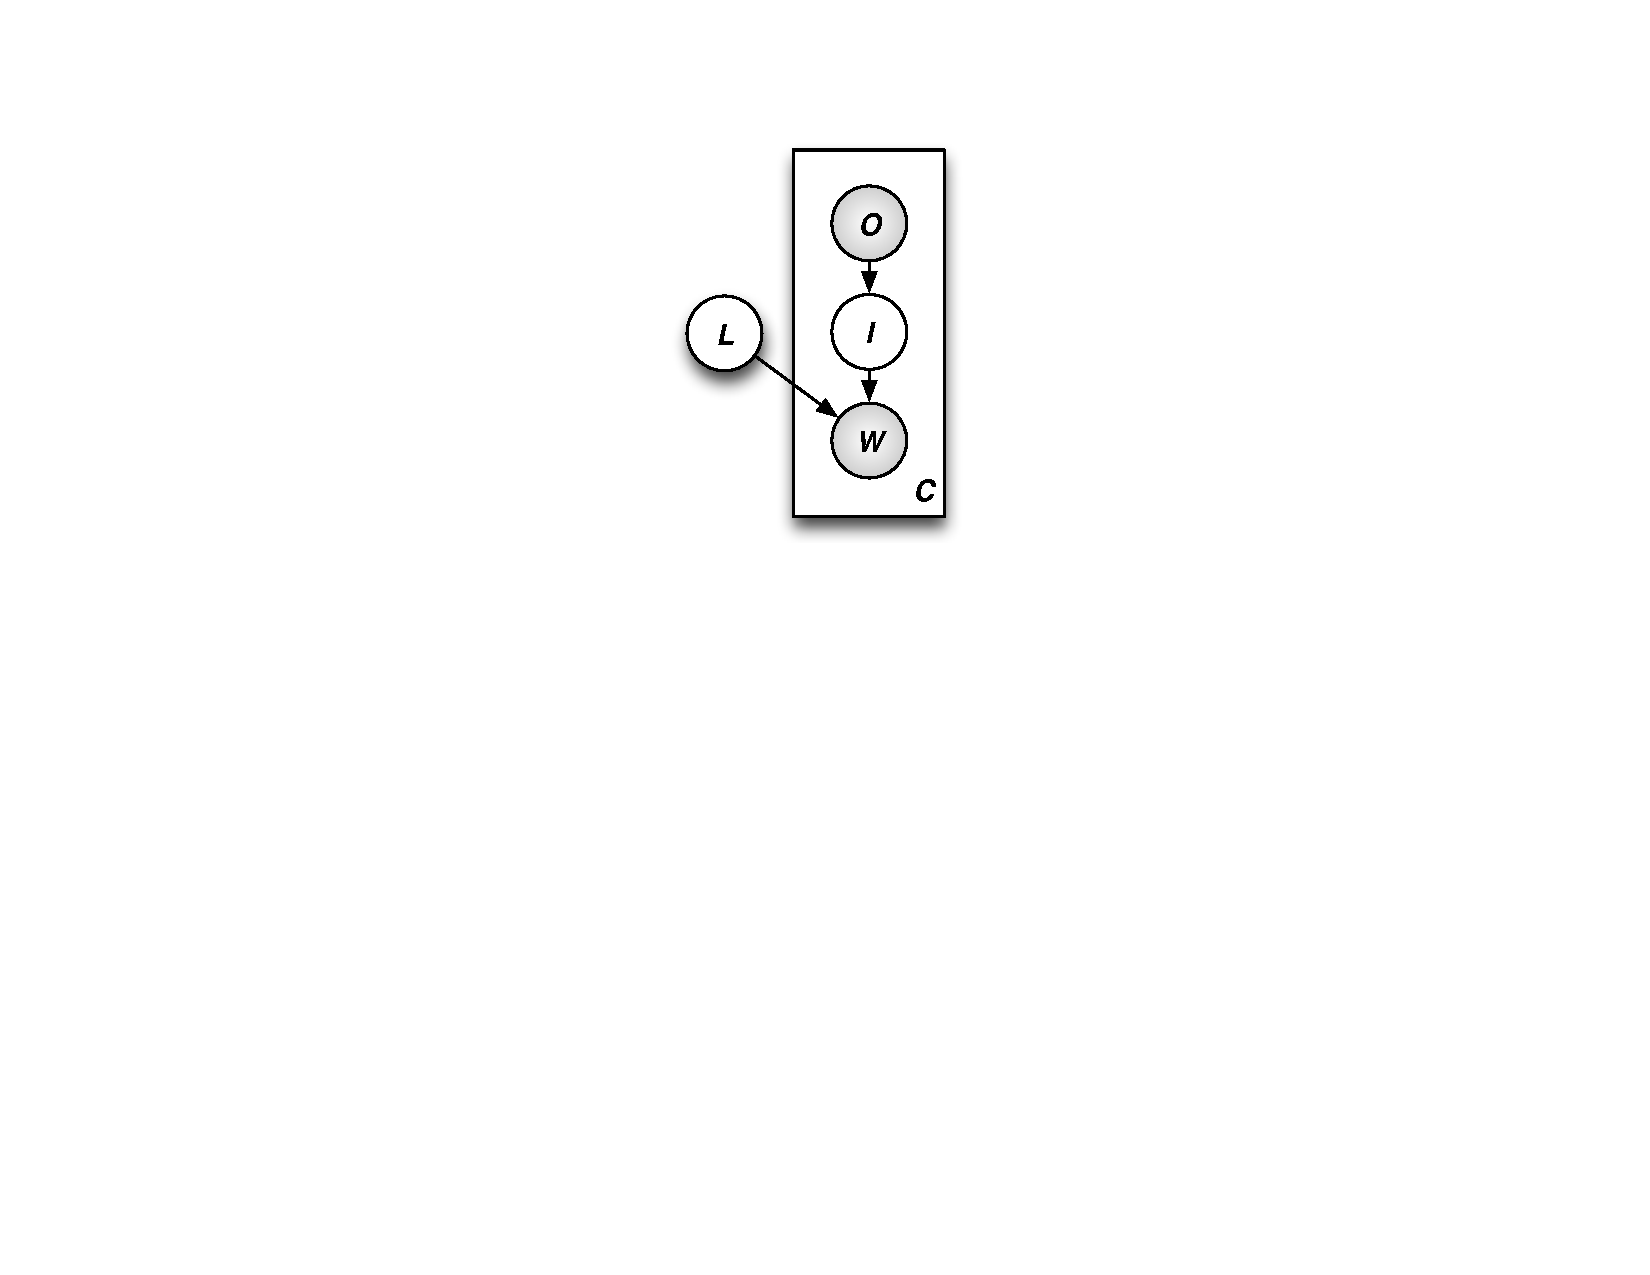
\includegraphics[width=1.5in]{figures/gen_mod.pdf}
\caption{\label{fig:genmod} The generative model assumed in both \protect\citeA{frank2009} and our current work. The plate over contexts indicates that objects, words, and referential intentions are present in each context, while the lexicon stays constant across contexts.}
\end{center}
\end{figure}

The learner can jointly infer $I$ and $L$ using Bayes' rule:

\begin{equation}
P( I, L | C) \propto P(C | I, L ) P(I, L).
\end{equation}

\noindent Because of the structure of the generative model shown in Figure \ref{fig:genmod}, we can replace contexts $C$ with the words and objects that constitute them:

% \begin{equation}
% P( I| W, O) \propto P(W | I, O) P(I).
% \end{equation}

\begin{equation}
P( I, L | W, O) \propto P(W, O | I, L) P(I, L).
\end{equation}


\noindent Objects $O$ are observed in the context, however, so can be removed. In addition, for simplicity, we assume that there is a uniform prior over possible intentions (though we return to this issue in the Discussion). Again by the generative model in Figure \ref{fig:genmod}, the remaining expression can be factored as follows:

\begin{equation}
P( I, L | W, O) \propto P(W | I, L) P(I | O) P(I) P(L).
\end{equation}

Here is where our current model diverges from that of \citeA{frank2009}. In that work, we integrated across referential intentions and focused primarily on inferring the meanings of words in the absence of further interpretive information. In contrast, in the current model we focus on the process of incremental interpretation, and treat the lexicon as a byproduct of the process of interpretation. Accordingly, we integrate over all possible lexicons:

\begin{equation}
P( I| W, O) \propto \int_L{P(W | I, L) P(I | O) P(I)  P(L) }
\end{equation}


Similarly to the previous work, we define the lexicon $L$ as consisting of two separate parts. The referential lexicon $L_R$ is a set of integrated Dirichlet-Multinomial distributions, one for each object in the world. This distribution represents the posterior probability of a particular word, relative to that object. The non-referential lexicon $L_{NR}$ is an independent Dirichlet-Multinomial distribution that captures the use of other words that do not refer in the current context.

\begin{equation}
P(L) = \prod_{o \in W}{P(L_{R_o})} + P(L_{NR}).
\end{equation}

 

% \begin{equation}
% P(W | I, L) = \gamma  
% \end{equation}

% intention, referential slot, and word vector
% for the referential word 

$p(\vect{w} | I, R, L_R, L_{NR}) = p(w|O_i) * prod_{s \in S - S_r} {P(W_s | L_{NR})}$

\subsection{Inference}
\begin{figure}[tr]
\begin{center}
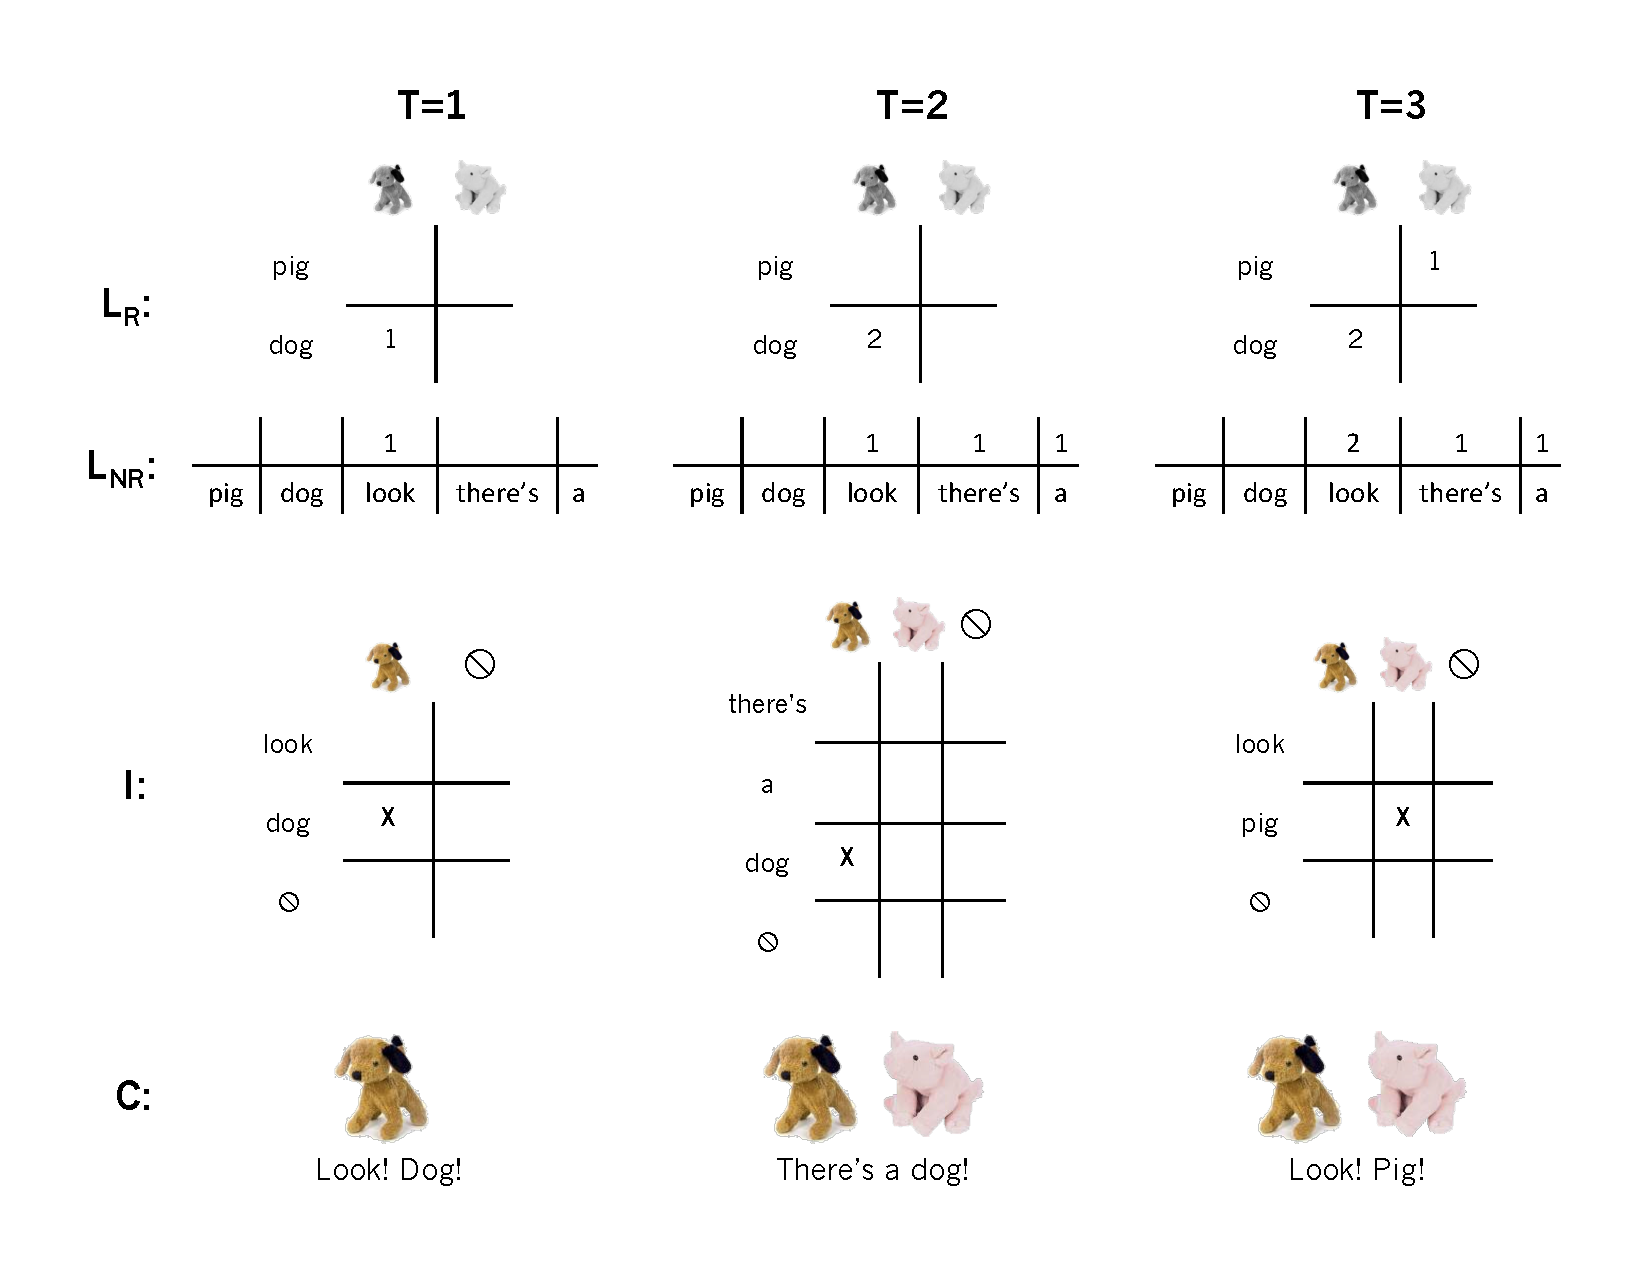
\includegraphics[width=6.5in]{figures/inference_diagram.pdf}
\caption{\label{fig:inference_diagram} Caption.}
\end{center}
\end{figure}

\subsubsection{Batch inference using a gibbs sampler}

\begin{equation}
P_t(L|W_{1...t}, O_{1...t}) \propto P_{t-1}(L | ...) P(W_t, I_t, R_t | L)
\end{equation}

% prob of a particular sample under Dir-M is the same thing as the conjugate 
% so you just get the conjugate update for each of the assignments 

\subsubsection{Incremental inference using a particle filter}

\begin{equation}
P_t(L|W_{1...t}, O_{1...t}) \propto P_{t-1}(L | ...) P(I_t | W_t, O_t)
\end{equation}

\section{Simulations}

\subsection{Corpus simulations}



\subsection{Cross-situational word learning with adults}

\subsubsection{Yu \& Smith (2007)}

\subsection{Experiments with children}

\subsubsection{Disambiguation}

\subsubsection{Dewar \& Xu (2007)}



\section{Discussion}



\subsection{Open questions for the cross-situational, social viewpoint}

\subsubsection{Synergies with other problems}

\subsubsection{Extensions to other parts of the vocabulary}

\subsubsection{Representations supporting cross-situational word learning}

\cite{yurovskyunderreview}

\subsection{Conclusions}

\newpage

\bibliographystyle{apacite}
\bibliography{dmww}

\end{document}

